
% --- SLIDE 6: EVIDENCE ---
\begin{frame}{Does It Actually Help? Yes, and Mostly Because of Pruning}

    \centering
    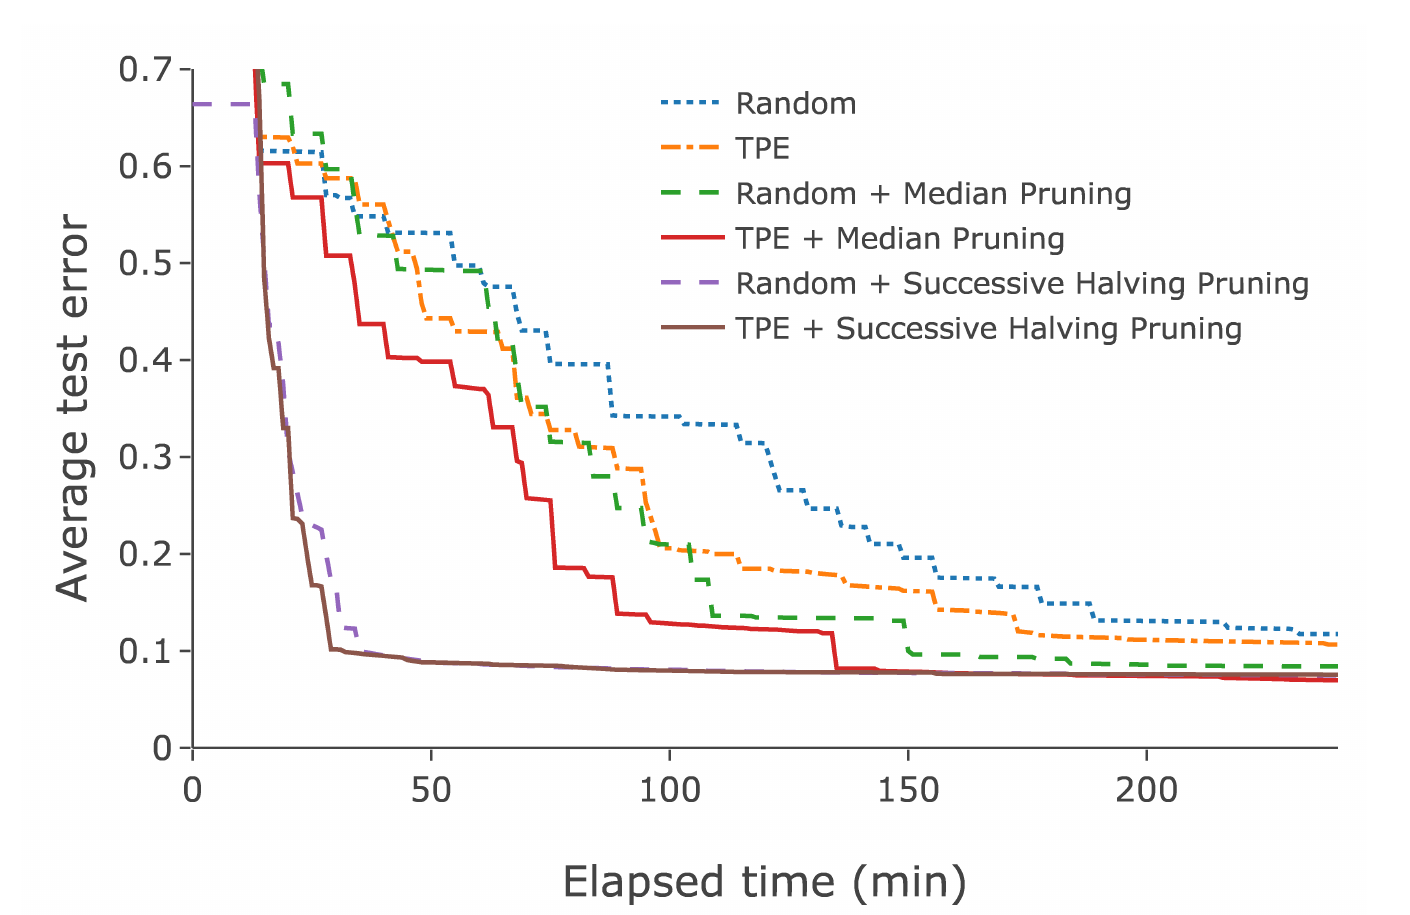
\includegraphics[width=0.62\textwidth,height=0.42\textheight,keepaspectratio]{images/mlops-foundations/optuna_pruning_test_error.png}

    {\scriptsize Source: Akiba, Sano, Yanase, Ohta \& Koyama, ``Optuna: A Next-generation Hyperparameter Optimization
    Framework,'' KDD 2019, \href{https://arxiv.org/abs/1907.10902v1}{arXiv:1907.10902v1}, Figure~11(a).
    Simplified AlexNet on SVHN; average test error against \emph{wall-clock} time.}

    \vspace{0.5em}
    \begin{itemize}
        \small
        \item Read the $x$-axis carefully: this is error against \textbf{elapsed time}, not against number of
              trials. That is the axis that costs money.
        \item TPE beats random search at equal time --- but the two curves that collapse almost immediately
              are the \textbf{pruned} ones. Pruning is the bigger win.
        \item In the same paper's RocksDB case study, a 4-hour budget explored \textbf{937} configurations
              with pruning versus \textbf{39} without.
    \end{itemize}

\end{frame}
